\graphicspath{ {imgs/} }
\documentclass[main.tex]{subfiles}
\begin{document}
\chapter{Model}\label{chap:model}
This section describes in detail the used model and the learning process that was used to train it.



\section{Architecture}

The network has two dense layers with $64$ neurons each. The activation function of the rectified linear unit is a simple maximum of the weighted inputs.

\begin{figure}
\begin{center}
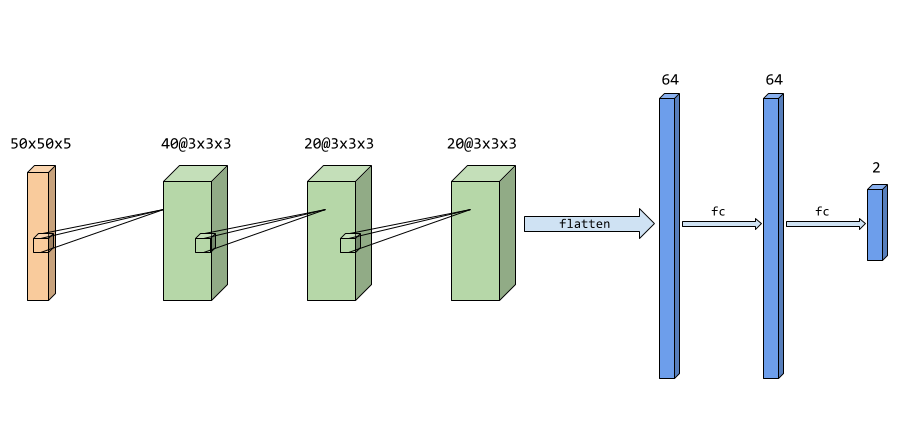
\includegraphics[scale=0.5]{net_struct.png}
\end{center}
\caption{Architecture of the neural network. Each of the convolutional layers is composed of a 3D convolution layer with the respective filter size followed by a batchnormalization and a pooling layer. The pool size is $(2,2,2)$ with a stride of $(1,1,1)$. The structure of the neural network resembles the one described by Huang~\cite{huang2017lung}.}
\label{fig:net_struct}
\end{figure}


\section{Training}
The input to the network are the slices that have been the result of the before described preprocessing and are fed to the network in batches. They are augmented by randomly flipping them in x and y plane (examples can be seen in \ref{fig:input}). The augmentation is applied to make the learned classification more robust against distortions in the input. It makes sense in this specific scenario since the nodules are growing in different shapes and locations in the lung and flipping them is not producing an impossible input to the network.

\begin{figure}
\begin{center}
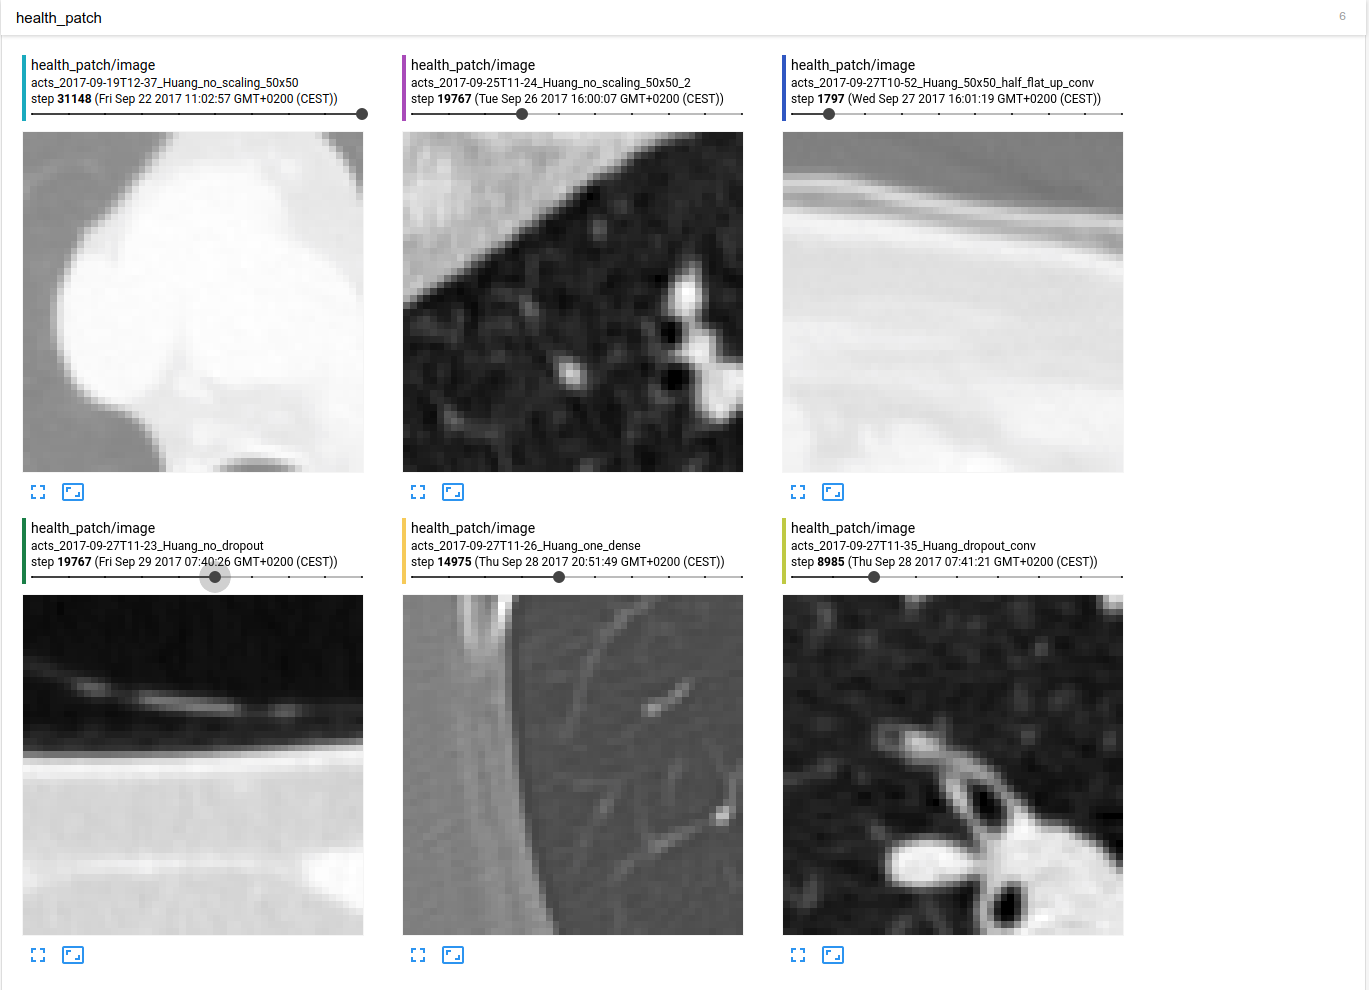
\includegraphics[scale=0.25]{patches-health.png}
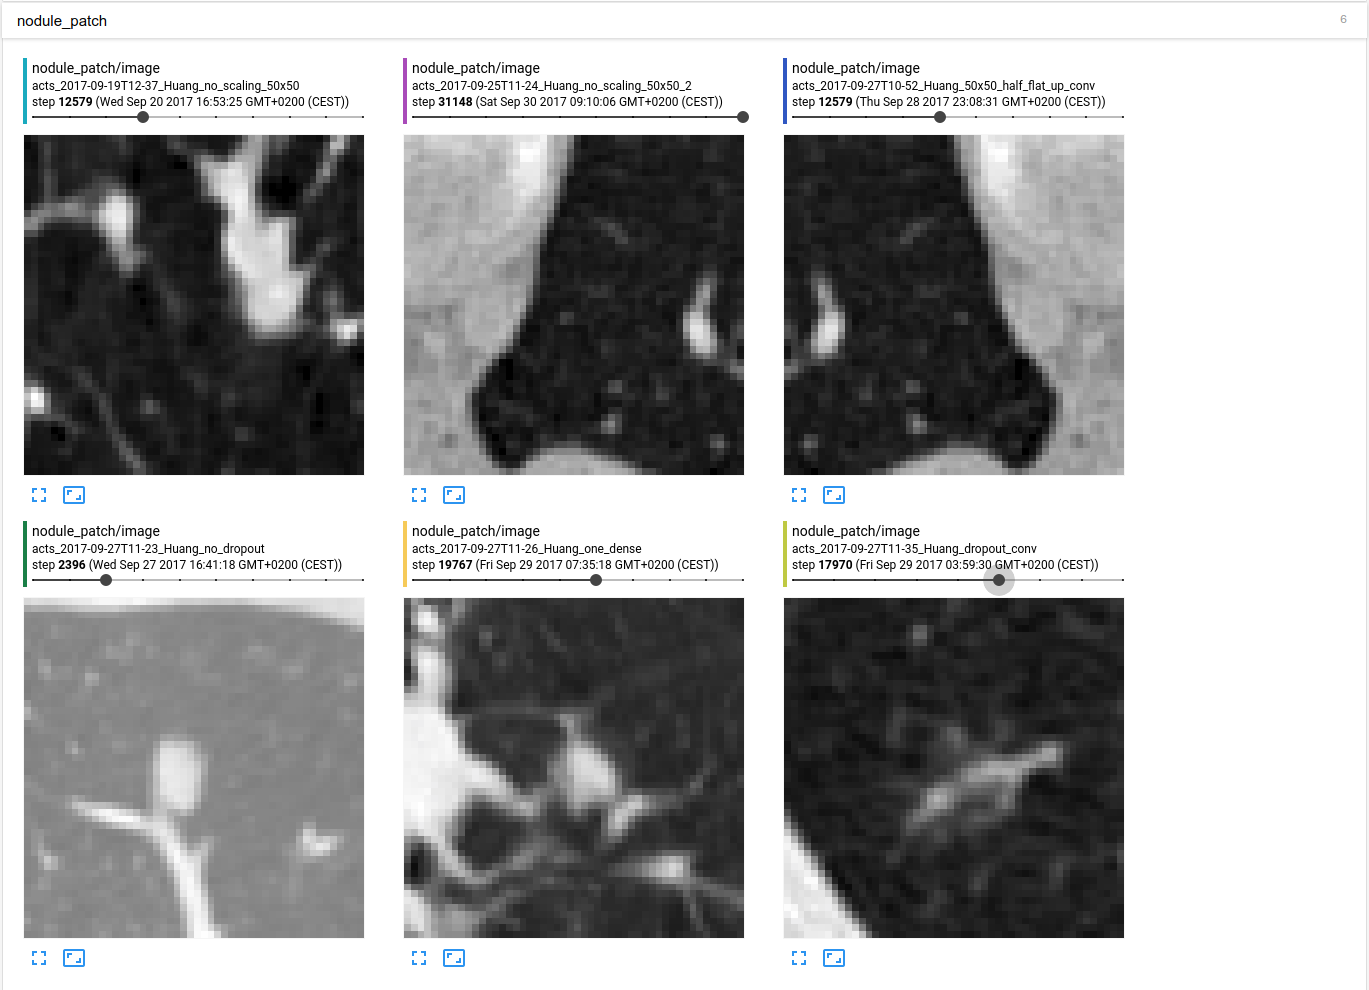
\includegraphics[scale=0.25]{patches-nodule.png}
\end{center}
\caption{Input data for the cases of healthy and nodule patches. The image is taken from Tensorboard and shows in the case of nodules the random permutation of the input data.}
\label{fig:input}
\end{figure}

Regularization methods used for this network include batchnormalization and dropout. Batchnormalizaton is in TensorFlow implemented as described by Ioffe and Szegedy~\cite{ioffe2015batch} and has been described already in section~\ref{ss:convlayer}. Dropout is another regularization method that was used in this thesis. It basically means that during training random neurons of the network are dropped - training effectively several models at once, as discovered by Srivastava et al.~\cite{srivastava2014dropout}, which should increase the overall performance of the network. During training no improved performance could be observed when applying dropout throughout the whole network. It was rather harmful if applied to the convolutional layers. The final model uses dropout only in the fully connected  layers.


\end{document}
